% Body of the article for the ReScience C template (article.tex inputs this file).
% Every number below is a macro generated by paper/build_tables.py from outputs/ and the repository
% docs; nothing numerical is typed by hand. Citations of the original give page and equation of
% Kim & Thorne (1991) [kim1991]. The scan of the original is not in the repository.
% Generated by paper/build_tables.py. Do not edit by hand.
\newcommand{\ArbiterRatioDev}{7.29\times10^{-19}}
\newcommand{\ArbiterXis}{0.5, 1.3, 2}
\newcommand{\BLarge}{0.01}
\newcommand{\BSmall}{10^{-6}}
\newcommand{\CodeCommit}{1e6e78aeac88}
\newcommand{\DbLarge}{0.01}
\newcommand{\DbSmall}{10^{-6}}
\newcommand{\DeltaLarge}{0.01}
\newcommand{\DeltaSmall}{10^{-6}}
\newcommand{\EpsLarge}{0.01}
\newcommand{\EpsSmall}{10^{-8}}
\newcommand{\FFiveEqFortyThree}{1.05\times10^{-80}}
\newcommand{\FFiveEqSixtyTwo}{1.81\times10^{-77}}
\newcommand{\FFiveFortyFourAMax}{4.87\times10^{-3}}
\newcommand{\FFiveFortyFourAMin}{8.68\times10^{-39}}
\newcommand{\FFiveLimitN}{60}
\newcommand{\FFourDevLarge}{7.76\times10^{-3}}
\newcommand{\FFourDevSmall}{7.76\times10^{-7}}
\newcommand{\FFourFD}{1.64\times10^{-16}}
\newcommand{\FFourHalfRatio}{0}
\newcommand{\FFourLiteralSmall}{0.578}
\newcommand{\FFourSlopeDev}{-9.6\times10^{-13}}
\newcommand{\FOneEqThirtyEightAtEight}{7.86\times10^{-9}}
\newcommand{\FOneEqThirtyEightAtTwo}{7.79\times10^{-3}}
\newcommand{\FOneEqThirtyFour}{1.48\times10^{-70}}
\newcommand{\FOneEqThirtyOne}{7.38\times10^{-80}}
\newcommand{\FOneEqThirtySeven}{1.46\times10^{-70}}
\newcommand{\FOneEqThirtyThree}{3.9\times10^{-70}}
\newcommand{\FOneEqTwentyNine}{2.11\times10^{-81}}
\newcommand{\FSevenPrinted}{10^{49}}
\newcommand{\FSevenRecomputed}{10^{59}}
\newcommand{\FSixEqFiftyFourFirst}{0.632}
\newcommand{\FSixEqFiftyFourFirstAt}{0.1}
\newcommand{\FSixEqFiftyFourLast}{9.07\times10^{-3}}
\newcommand{\FSixEqFiftyFourLastAt}{0.001}
\newcommand{\FSixEqFiftyThree}{1.25\times10^{-9}}
\newcommand{\FSixEqSixtyEight}{5.34\times10^{-11}}
\newcommand{\FSixEqSixtyNine}{1.99\times10^{-8}}
\newcommand{\FThreeDevLarge}{4.04\times10^{-3}}
\newcommand{\FThreeDevSmall}{4.04\times10^{-7}}
\newcommand{\FThreeFD}{3.96\times10^{-20}}
\newcommand{\FThreeHalfSmall}{1.01\times10^{-7}}
\newcommand{\FThreeOffAxisMax}{4.95\times10^{-3}}
\newcommand{\FThreeSlopeDev}{-4.39\times10^{-6}}
\newcommand{\FThreeSlopeHalfDev}{-4.39\times10^{-6}}
\newcommand{\FThreeX}{0.25}
\newcommand{\FThreeXHalf}{0.5}
\newcommand{\FTwoBetweenLarge}{0.0639}
\newcommand{\FTwoBetweenSmall}{6.67\times10^{-6}}
\newcommand{\FTwoLapse}{4.22\times10^{-81}}
\newcommand{\FTwoThroatLarge}{0.0389}
\newcommand{\FTwoThroatSmall}{4.0\times10^{-6}}
\newcommand{\LitArxiv}{131}
\newcommand{\LitCiting}{175}
\newcommand{\LitMention}{99}
\newcommand{\LitMissing}{44}
\newcommand{\ModesMaxDiff}{2.51\times10^{-8}}
\newcommand{\PhaseOnePoints}{15}
\newcommand{\PhaseOneSlopeDev}{-3.84\times10^{-15}}
\newcommand{\PhaseOneTwoPiMax}{3.17\times10^{-22}}
\newcommand{\PhaseOneWorst}{5.5\times10^{-16}}
\newcommand{\ThermalEqFourA}{1.9999999999999999999}
\newcommand{\ThermalFDErr}{3.16\times10^{-20}}
\newcommand{\ThermalHalf}{0.99999999999999999997}
\newcommand{\ThermalPressureDev}{2.5\times10^{-20}}
\newcommand{\ThermalTemps}{0.3, 1, 3}
\newcommand{\ThermalTrace}{8.36\times10^{-23}}
\newcommand{\TranscribedEquations}{52}
\newcommand{\UnruhEqFourADev}{10^{-19}}
\newcommand{\UnruhHalfDev}{6.0\times10^{-20}}
\newcommand{\VersionMatplotlib}{3.11.2}
\newcommand{\VersionMpmath}{1.4.1}
\newcommand{\VersionNumpy}{2.5.4}
\newcommand{\VersionPython}{3.13.13}
\newcommand{\WorkingDigits}{80}


\section{Introduction}

Kim and Thorne~\cite{kim1991} asked whether vacuum fluctuations of a quantum field destroy a wormhole time machine before closed timelike curves can form. They modelled the time machine as a wormhole whose two mouths, at rest separation $D$ and with throat radius $b \ll D$, are set in relative motion, so that a Cauchy horizon forms. On this background they computed the renormalized stress-energy tensor $\langle T^{\mu\nu}\rangle$ of a conformally coupled massless scalar field. The calculation is semiclassical: the field is quantized on a fixed spacetime.
\begin{itemize}
\item \textbf{The divergence.} The tensor grows without bound near the Cauchy horizon, as the inverse cube of the distance to it, both at the throat (eq.~51, p.~3943) and between the mouths (eq.~67, p.~3945).
\item \textbf{The cutoff.} Kim and Thorne argued that quantum gravity plausibly cuts the growth off when the proper time to the horizon reaches the Planck time, $\Delta t \sim l_P$ (eqs.~9--14 and the surrounding text, pp.~3934--3937). At that point the metric perturbation is still tiny, so vacuum polarization would not prevent the time machine from forming.
\item \textbf{Hawking's objection.} Hawking~\cite{hawking1992}, in the paper that states the chronology protection conjecture, disputed this cutoff (p.~603 and section~VI). He argued that a cutoff should be imposed on an invariant distance rather than on an observer-dependent proper time, which corresponds to $D\,\Delta t \sim l_P^2$, where the perturbation reaches order unity.
\item \textbf{The limit of the semiclassical approach.} Kay, Radzikowski and Wald~\cite{krw1997} later showed that the two-point function cannot be of Hadamard form on a compactly generated Cauchy horizon, so the question cannot be settled within the semiclassical framework.
\end{itemize}

\paragraph{What is replicated.} This paper replicates the \emph{computational} content of Kim and Thorne's article. The article derives closed-form results from a small set of starting expressions:
\begin{itemize}
\item the identification map of the wormhole (eqs.~25 and 28);
\item the Hadamard function as a sum over closed geodesics (eq.~20) and its geometric-optics form at the throat (eqs.~46 and 50) and between the mouths (eqs.~61 and 66);
\item the point-splitting operator (eqs.~4a and 4b).
\end{itemize}
Every closed form that follows from these is recomputed here by a different numerical route, in arbitrary-precision arithmetic, and compared with the printed result. The closed forms are the covering-space geometry, the defocusing factors, the stress-energy, the polarized hypersurfaces and the four-momentum. This is replication in the sense of ReScience: the derivations are repeated with different technical means (direct numerical evaluation instead of analytic expansion) and checked against the printed numbers and formulas.

The replication does not test whether the starting expressions describe the physical system correctly, since they are inputs. Nor does it take a side between Kim and Thorne and Hawking.

\section{Previous work on the same result}
\label{sec:previous}

Two later works recompute the analogue of one of Kim and Thorne's results.
\begin{itemize}
\item \textbf{Klinkhammer (1992), PhD thesis~\cite{klinkhammer1992}.}
  \begin{itemize}
  \item He derives the stress-energy near a closed null geodesic for multiply connected spacetimes (eqs.~3.7 and 3.8, pp.~31--32 of the thesis), using an operator (eq.~3.3, p.~30) that equals the operator of Kim and Thorne's eq.~4b multiplied by $\tfrac12$.
  \item With Kim and Thorne's van Vleck factor (eq.~64) and $e^h = 1/\xi$ (eq.~33), his eq.~3.8 is \emph{exactly half} of Kim and Thorne's eq.~67. This is an algebraic identity, checked by a test in the repository.
  \item He states that their results ``are in perfect agreement with ours'' (thesis, section~4, p.~38). He does not comment on the factor.
  \end{itemize}
\item \textbf{Visser, arXiv:hep-th/9303023~\cite{visser1993}.}
  \begin{itemize}
  \item He uses the same operator as Klinkhammer (his eq.~10) and obtains Klinkhammer's result (his eq.~34).
  \item He states that it ``is consistent with that of Kim and Thorne~[3] --- their equation~(67).'' He does not comment on the factor either.
  \end{itemize}
\end{itemize}
Both works therefore recompute only the analogue of eq.~67, obtain half of it, and cover none of the other results replicated here (F1--F7 below). Two limits apply to this comparison. Both transcriptions come from a single reading. The published version of Klinkhammer's work, which Visser cites as Phys.\ Rev.\ D 46, 3388 (1992), was not read.

\section{Methods}

\subsection{Independent re-implementation}

The code (\texttt{chronosim}, Python with the arbitrary-precision library mpmath) never uses a closed form to compute its own check. Each result is reached by a different route:
\begin{itemize}
\item \textbf{Covering space:} built by iterating the identification map of eqs.~25 and 28, without eqs.~29--38.
\item \textbf{Stress-energy:} obtained by applying the point-splitting operator, as finite differences, to the regularized Hadamard functions of eqs.~50 and 66 (with $\lambda_N$ from eqs.~46 and 61), without eqs.~51 and 67.
\item \textbf{Defocusing factors:} computed from ray-transfer matrices of the thin divergent lens that the text describes (p.~3942), without eqs.~47, 48 and 64.
\item \textbf{Polarized hypersurfaces:} found as roots of $\lambda_N(x,x) = 0$.
\item \textbf{Four-momentum:} obtained by quadrature of eqs.~51 and 67 on the domains written in the article.
\end{itemize}
Two operators run in parallel throughout: eq.~4a as printed, and the same operator multiplied by $\tfrac12$. Units are $\hbar = c = 1$ and $D = 1$ unless stated. The working precision is \WorkingDigits{} decimal digits (a \textsc{heuristic} choice).

\subsection{Provenance by construction}

Every number the code emits is a \texttt{Quantity} that carries an origin:
\begin{itemize}
\item \textsc{cited}: transcribed from a source;
\item \textsc{derived}: evaluated exactly from cited formulas;
\item \textsc{computed}: produced by a numerical procedure;
\item \textsc{heuristic}: chosen without a source, such as a step size or a series cutoff.
\end{itemize}
Combining quantities yields the worst origin among the inputs, and no code path promotes a value to a better origin. Every heuristic constant is registered and printed on every run. A test (\texttt{tests/test\_anti\_fabrication.py}) fails if any module of the package can reach a random number generator; sampling uses deterministic grids only.

\subsection{Transcription of the scanned original}
\label{sec:transcription}

The PDF of the original is a scan without extractable text.
\begin{itemize}
\item \textbf{Two passes.} Every equation used was transcribed twice, in separate passes from enlarged crops. The second pass was done by a separate model instance with no access to the first. All \TranscribedEquations{} equations agree between the passes (record in \texttt{docs/equation\_transcription.md}).
\item \textbf{Limitation.} Both passes come from the same kind of model, so they are not two independent human readers. A reading error common to both would not be detected by this comparison. This is one reason why the derivations of F3 and F4 below also act as a check.
\item \textbf{Third, human reading.} The author checked the following against the scan:
  \begin{itemize}
  \item eqs.~1, 3, 4a and 4b (pp.~3932--3933);
  \item eq.~31 (p.~3940);
  \item eq.~52 (p.~3943);
  \item the text after eq.~14 (p.~3935), together with the value of $m_P$ after eq.~54 (p.~3943).
  \end{itemize}
  The value of $l_P$ on p.~3930 was not checked by the author (section~\ref{sec:limitations}).
\end{itemize}

\subsection{Arbiters for the point-splitting operator}
\label{sec:arbiters}

The operator is anchored by references that do not depend on Kim and Thorne.
\begin{itemize}
\item \textbf{Primary arbiter: a thermal state in Minkowski space.}
  \begin{itemize}
  \item The Hadamard function is the image sum in imaginary time, derived from the KMS condition (written out in \texttt{docs/thermal\_images.md}), with the Minkowski-vacuum term removed.
  \item The reference is the Stefan--Boltzmann density of a massless scalar, $\pi^2T^4/30$, cross-checked against the Bose integral.
  \item The image sum was also compared with the mode integral with Bose occupation numbers, at separated points: the largest relative difference is $\ModesMaxDiff$, and it comes from truncating the image sum.
  \end{itemize}
\item \textbf{Secondary arbiter: the Unruh value in the Rindler vacuum,} $\rho = -\pi^2T^4/30$ with $T = 1/(2\pi\xi)$. This reference is labelled \textsc{heuristic}: the relation is cited from Candelas and Deutsch~\cite{candelas1977}, which was not read (closed access; volume and pages confirmed in Crossref only).
\item \textbf{Direct comparison} of eq.~4a with eq.~11 of Li and Gott~\cite{ligott1998} (arXiv version, p.~2), on the Rindler function. Both articles normalize the Hadamard function identically: $1/(4\pi^2\sigma)$, with $\sigma$ half the squared separation (Kim and Thorne eqs.~3, 17 and 20; Li and Gott eq.~9). Li and Gott's eq.~11 has the coefficients of eq.~4b and an overall $\tfrac12$.
\end{itemize}

\subsection{Validation of the method on Li and Gott (1998)}

Before the wormhole, the same machinery was validated on Misner space against Li and Gott~\cite{ligott1998}. The image sum (their eq.~8), with point splitting (their eq.~11), was compared with their closed form (their eq.~12) on $\PhaseOnePoints$ points, four components each.
\begin{itemize}
\item \textbf{Agreement:} the largest difference, relative to the scale $1/(1440\pi^2\xi^4)$, is $\PhaseOneWorst$ (\textsc{computed}).
\item \textbf{Horizon slope:} the log--log slope of $|\rho|$ against $\xi$ differs from the $-4$ that eq.~12 predicts by $\PhaseOneSlopeDev$.
\item \textbf{The self-consistent value $b = 2\pi$}, where eq.~12 vanishes: the largest computed $|\rho|$ there is $\PhaseOneTwoPiMax$.
\end{itemize}
Figure~\ref{fig:phase1} shows the horizon divergence.

\begin{figure}[t]
\centering
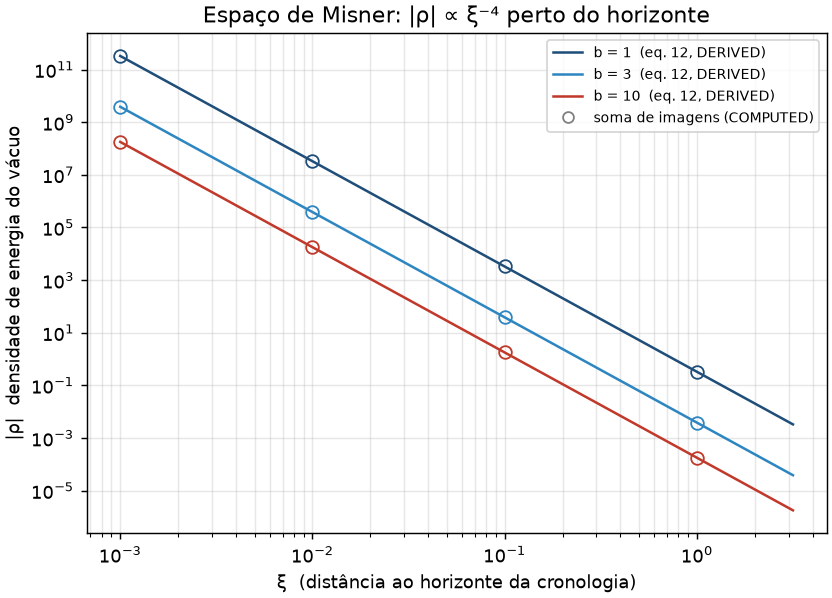
\includegraphics[width=0.7\linewidth]{../outputs/fig1_horizon_divergence.png}
\caption{Method validation on Misner space: image sum with point splitting (Li and Gott eqs.~8 and 11) against their closed form (eq.~12), near the chronology horizon. \textsc{computed} against \textsc{derived}. The labels of this figure are in Portuguese; see section~\ref{sec:limitations}.}
\label{fig:phase1}
\end{figure}

\section{Results}

Table~\ref{tab:results} summarizes items F1--F7. The points below it give the context a table cannot.

\begin{table}[t]
\centering\small
\begin{tabular}{p{0.07\linewidth}p{0.36\linewidth}p{0.47\linewidth}}
\toprule
Item & Claim of the original (page, equation) & Independent computation and measured agreement (all \textsc{computed}) \\
\midrule
F1 & Covering space: origin (eq.~29), copies (eq.~33), $\sigma_N$ (eq.~34), $\Delta U$ (eq.~37), pp.~3940--3941 & Iterated identification map. Largest deviations $\FOneEqTwentyNine$, $\FOneEqThirtyThree$, $\FOneEqThirtyFour$, $\FOneEqThirtySeven$. \\
F1 & Approximate interval, eq.~38 (p.~3941) & Relative error against the exact interval: $\FOneEqThirtyEightAtTwo$ at $\epsilon/D = \EpsLarge$, $\FOneEqThirtyEightAtEight$ at $\EpsSmall$; first order in $\epsilon$ (our measurement; the article states no order). \\
F2 & Defocusing, eqs.~47, 48, 64 (pp.~3942, 3945) & Thin-lens ray transfer. Largest relative deviation $\FTwoThroatLarge$ (throat) and $\FTwoBetweenLarge$ (between) at $b/D = \BLarge$; $\FTwoThroatSmall$ and $\FTwoBetweenSmall$ at $\BSmall$. \\
F2 & Lapse, eq.~57 (p.~3944) & Against the exact lapse from the covering space: $\FTwoLapse$. \\
F3 & $\langle T^{\mu\nu}\rangle$ between the mouths, eq.~67 (p.~3945) & Finite differences on eq.~66 with the operator as printed. On the axis, largest deviation $\FThreeDevLarge$ at $\Delta/D = \DeltaLarge$ and $\FThreeDevSmall$ at $\DeltaSmall$. Off the axis, up to $\FThreeOffAxisMax$. With $\tfrac12$: ratio $\tfrac12$ to within $\FThreeHalfSmall$. Slope $-3$ to within $\FThreeSlopeDev$. \\
F4 & $\langle T^{\mu\nu}\rangle$ at the throat, eq.~51 (p.~3943) & Finite differences on eq.~50 with the operator as printed and $\hat\rho$ from $\rho=\sqrt{Y^2+Z^2}$. Largest deviation $\FFourDevLarge$ at $\Delta/b = \DbLarge$ and $\FFourDevSmall$ at $\DbSmall$. With $\tfrac12$: ratio $\tfrac12$ in every digit stored ($\FFourHalfRatio$ difference). Slope $-3$ to within $\FFourSlopeDev$. \\
F5 & Polarized hypersurfaces and Cauchy horizon, eqs.~43, 44a, 62, 63 (pp.~3941, 3944) & Roots of $\lambda_N(x,x)=0$. Largest deviations $\FFiveEqFortyThree$ (eq.~43) and $\FFiveEqSixtyTwo$ (eq.~62). At $N = \FFiveLimitN$, eq.~44a is approached to within $\FFiveFortyFourAMin$--$\FFiveFortyFourAMax$, like $\xi^N$. \\
F6 & Four-momentum, eqs.~53, 54, 68, 69 (pp.~3943, 3945--3946) & Quadrature of eqs.~51 and 67. Eq.~69: $\FSixEqSixtyNine$. Eq.~68: $\FSixEqSixtyEight$. Eq.~54, a leading term: $\FSixEqFiftyFourFirst$ at $\Delta T/b = \FSixEqFiftyFourFirstAt$ down to $\FSixEqFiftyFourLast$ at $\FSixEqFiftyFourLastAt$. Coefficient of $\ln(b/a)$ in eq.~53: $\FSixEqFiftyThree$. \\
F7 & Order-of-magnitude estimates, eqs.~9, 13, 14 (pp.~3934--3937) & Arithmetic from the inputs printed in the article: Table~\ref{tab:f7}. Only the arithmetic is checked, not the estimates. \\
\bottomrule
\end{tabular}
\caption{Results of the replication. Deviations are relative, against the printed closed form. F3, F4 and F6 use the operator of eq.~4a as printed; with $\tfrac12$ every stress-energy value is half as large.}
\label{tab:results}
\end{table}

\begin{itemize}
\item \textbf{The residuals have the form of the neglected terms.}
  \begin{itemize}
  \item At the throat (F4), the residual falls linearly with $\Delta/b$. It is the term with the transverse second derivatives of $\lambda_N$, which eq.~51 does not contain: its analytic expression reproduces the residual in the $YY$, $YZ$ and $ZZ$ components, and the other components sit at the level of the numerical error.
  \item Between the mouths (F3), the residual falls linearly with $\Delta$ on the axis at $X/D = \FThreeX$. At $X/D = \FThreeXHalf$ the first derivative of the prefactor of eq.~66 vanishes: $T^{TT}$ and $T^{TX}$ sit at the level of the numerical error, and only $T^{XX}$ deviates, quadratically. Off the axis it grows like $(\rho/X)^2$ in the $kk$ component and like $\rho/X$ in the others: the fractional correction the text says it ignores (p.~3945).
  \end{itemize}
  This is the main reason to regard the closed forms as replicated, rather than merely approximated.
\item \textbf{The $\Delta^{-3}$ rate} (slope $-3$) is independent of the operator's normalization.
\item \textbf{Numerical error.} The largest finite-difference error estimates are $\FThreeFD$ (F3) and $\FFourFD$ (F4), far below every deviation in the table.
\item \textbf{Figures.} Figure~\ref{fig:divergence} shows the divergence with both operators, and Figure~\ref{fig:cutoffs} shows the two proposed cutoffs side by side.
\end{itemize}

\begin{figure}[t]
\centering
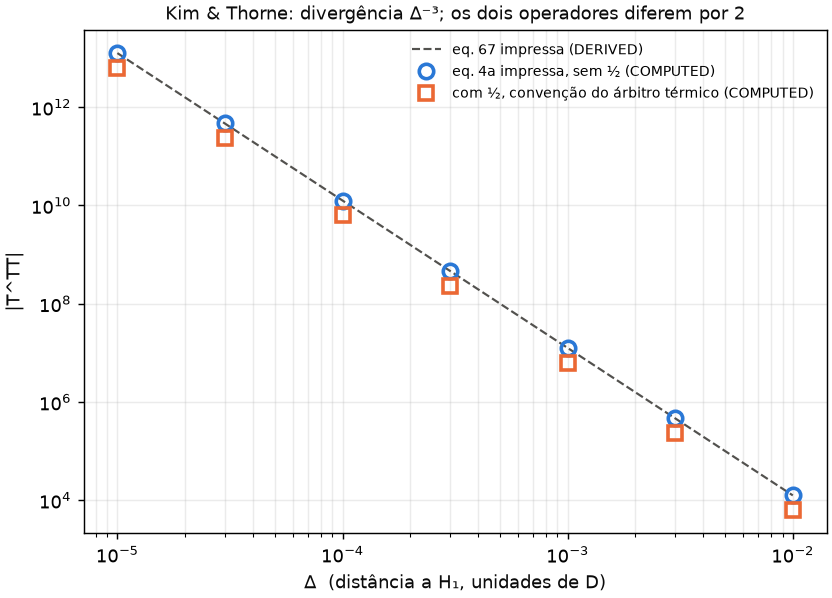
\includegraphics[width=0.7\linewidth]{../outputs/fig3_kt_divergence.png}
\caption{$|T^{TT}|$ between the mouths against the distance $\Delta$ to the first polarized hypersurface. Dashed: eq.~67 as printed. Circles: the operator of eq.~4a as printed. Squares: the operator with $\tfrac12$. All \textsc{computed}. The labels of this figure are in Portuguese; see section~\ref{sec:limitations}.}
\label{fig:divergence}
\end{figure}

\begin{figure}[t]
\centering
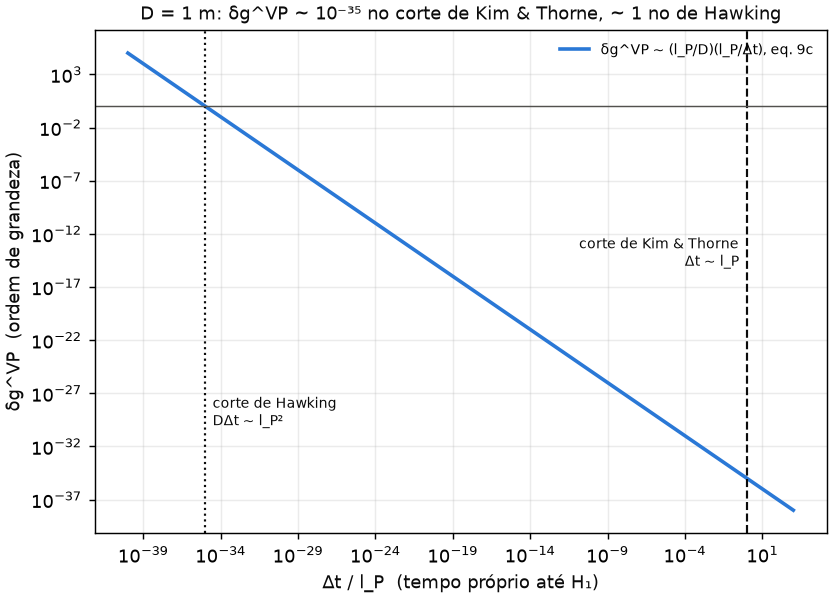
\includegraphics[width=0.7\linewidth]{../outputs/fig4_kt_cutoffs.png}
\caption{Metric perturbation $\delta g^{VP}$ against $\Delta t$, with the cutoff of Kim and Thorne ($\Delta t \sim l_P$, pp.~3934--3937) and that of Hawking ($D\,\Delta t \sim l_P^2$, Hawking 1992, p.~603 and section~VI). The figure shows both and does not choose between them. The labels of this figure are in Portuguese; see section~\ref{sec:limitations}.}
\label{fig:cutoffs}
\end{figure}

\section{Discrepancies}
\label{sec:discrepancies}

For each discrepancy, the subsection gives what is printed, what the computation shows, and what depends on it.

\subsection{Normalization of the point-splitting operator (eq.~4a)}

\begin{itemize}
\item \textbf{What is printed.}
  \begin{itemize}
  \item Eq.~4a (p.~3933) defines $T_{\mu\nu} = \lim_{x\to x'} D_{\mu\nu} G^{(1)}_{\rm reg}$.
  \item Eq.~4b gives $D_{\mu\nu} = \tfrac23\nabla_\mu\nabla_{\nu'} - \tfrac13\nabla_\mu\nabla_\nu - \tfrac16 g_{\mu\nu}\nabla_\alpha\nabla^{\alpha'}$, with no overall $\tfrac12$.
  \item The definitions around it were read with that question in mind: $G^{(1)}$ as the expectation of two field products (eq.~1), the subtraction $1/(4\pi^2\sigma_0)$ (eq.~3) and the normalization of eqs.~17 and~20.
  \item None of them supplies a compensating factor, and the author's reading of eqs.~1, 3, 4a and 4b confirms the transcription.
  \end{itemize}
\item \textbf{What the arbiters show.} With $\tfrac12$ the operator reproduces Stefan--Boltzmann and the Unruh value; as printed it gives twice both (Table~\ref{tab:arbiters}). The thermal state also has pressure $\rho/3$ to within $\ThermalPressureDev$ and trace $\ThermalTrace$ relative to $\rho$, for temperatures $T = \ThermalTemps$. Against Li and Gott's eq.~11 the ratio is $2$ to within $\ArbiterRatioDev$ at $\xi = \ArbiterXis$.
\item \textbf{What the printed results carry.} Eqs.~51 and 67 are reproduced \emph{by the operator as printed} (F3, F4). The normalization of eq.~4a is therefore carried consistently through to the final results, and the printed stress-energy values lie a factor of two above the convention that matches the arbiters.
\end{itemize}

\begin{table}[t]
\centering\small
% Generated by paper/build_tables.py from outputs/kt_thermal_arbiter.csv, kt_unruh_arbiter.csv, kt_arbiter_eq4a_vs_eq11.csv.
\begin{tabular}{p{0.17\linewidth}p{0.20\linewidth}ll}
\toprule
Reference & Origin of the reference & eq.~4a as printed & with $\tfrac12$ \\
\midrule
Stefan--Boltzmann, $\rho/(\pi^2T^4/30)$, $T=1$ & closed form, checked by the Bose integral (COMPUTED) & $1.9999999999999999999$ & $0.99999999999999999997$ \\
Unruh, $\rho/\rho_{\rm ref}$, $\xi=0.5$ & HEURISTIC (source not read) & $1.9999999999999999999$ & $0.99999999999999999994$ \\
Li \& Gott eq.~11 (validated in phase 1), $\xi=0.5$ & COMPUTED & $2.0$ & --- (reference) \\
\bottomrule
\end{tabular}

\caption{The operator against references that do not depend on Kim and Thorne. Ratios of the computed density to the reference. The thermal reference is the Stefan--Boltzmann law, checked against a numerical Bose integral; the image sum it is compared with comes from a derivation written out in the repository. The Unruh reference is \textsc{heuristic} because its source was not read.}
\label{tab:arbiters}
\end{table}

\subsection{Eq.~31 (p.~3940)}

\begin{itemize}
\item \textbf{What is printed.} Eq.~31 reads $\tilde T + \xi^n D/(1-\xi) = \frac{1+\xi^{2n}}{1-\xi^{2n}}\,(\tilde X + \xi^n D/(1-\xi))$. The positive sign of the coefficient was confirmed by the author.
\item \textbf{What the construction shows.} The covering space built from eqs.~25, 28 and 29 gives the coefficient with the opposite sign: the ratio to the printed coefficient is $-1$ to within $\FOneEqThirtyOne$.
\item \textbf{Fig.~5} draws the copies $n \geq 1$ with negative slope, whereas the printed eq.~31 gives a positive slope for $0<\xi<1$.
\item \textbf{What does not distinguish the sign.} Two other features of Fig.~5 do not distinguish it: the position of $T_0$, and the horizon crossings with spacings $D$, $D\xi$, $D\xi^2$.
\item \textbf{What depends on it.} No later result of the article depends on this equation.
\end{itemize}

\subsection{Eq.~52 (p.~3943)}

\begin{itemize}
\item \textbf{What is printed.} The unit transverse vector reads $\hat\rho = \partial/\partial\rho = (X^2+Y^2)^{-1/2}(Y\partial_Y + Z\partial_Z)$. The author confirmed the radicand $X^2+Y^2$.
\item \textbf{What is inconsistent with it.} The printed form disagrees with four things:
  \begin{itemize}
  \item the definition $\rho = \sqrt{Y^2+Z^2}$ (eq.~39);
  \item the equality $\hat\rho = \partial/\partial\rho$ within the same equation;
  \item the text, which calls $\hat\rho$ a unit vector (p.~3943);
  \item eq.~51 itself.
  \end{itemize}
  Eq.~51 is reproduced only with $\sqrt{Y^2+Z^2}$. With the printed radicand, the deviation is $\FFourLiteralSmall$ at $\Delta/b = \DbSmall$ and does not fall with $\Delta$. The text after eq.~52 also refers to ``the stress-energy tensor~(52)'', meaning eq.~51.
\end{itemize}

\subsection{The value after eq.~14 (p.~3935)}

\begin{itemize}
\item \textbf{What is printed.} The text gives $T^{00}_{\max} \sim (l_P/D)(m_P/l_P^3)$ (eq.~14) and the value $\sim \FSevenPrinted$\,g/cm$^3$.
\item \textbf{What the printed inputs give.} With the inputs the article itself prints beside it, $m_P$ after eq.~54 (p.~3943) and $l_P/D$ with $D = 1$\,m (p.~3935), the expression gives $\sim \FSevenRecomputed$\,g/cm$^3$ (Table~\ref{tab:f7}). The other estimates are consistent.
\item \textbf{Reading.} The author's reading of the printed exponent is unambiguous.
\item \textbf{What depends on it.} This is an order-of-magnitude estimate, and no conclusion of the article depends on it.
\end{itemize}

\begin{table}[t]
\centering\small
% Generated by paper/build_tables.py from outputs/kim_thorne_f7.csv.
\begin{tabular}{lll}
\toprule
Quantity & Printed (CITED) & Recomputed (DERIVED) \\
\midrule
$l_P/D$, $D = 1$\,m & $10^{-35}$ & $10^{-35}$ \\
$(\delta L/L)_{\max}$, eq.~13 & $10^{-35}$ & $10^{-35}$ \\
Planck density $m_P/l_P^3$ & $10^{94}$\,g/cm$^3$ & $10^{94}$\,g/cm$^3$ \\
$T^{00}_{\max}$, eq.~14 & $10^{49}$\,g/cm$^3$ & $10^{59}$\,g/cm$^3$ \\
Hawking cutoff $\Delta t$ ($\delta g^{VP}=1$, eq.~9c) & $10^{-35}$\,$l_P$ & $10^{-35}$\,$l_P$ \\
\bottomrule
\end{tabular}

\caption{F7: printed estimates against the arithmetic of the inputs printed with them.}
\label{tab:f7}
\end{table}

\section{Discussion}

\paragraph{Why the factor of two is a normalization issue, not a failure of replication.}
\begin{itemize}
\item \textbf{The question a replication asks:} whether the article's results follow from its stated starting points by its stated methods. For every closed form examined here they do: eqs.~51 and 67 follow from eqs.~50 and 66 through the operator of eq.~4a exactly as printed.
\item \textbf{What the factor is.} It sits in one overall constant, the normalization of the operator relative to the normalization of $G^{(1)}$. That constant multiplies every stress-energy value of the article uniformly.
\item \textbf{What the arbiters decide.} They decide which value of the constant reproduces known physics (a thermal state, the Unruh value, Li and Gott's operator): the value with $\tfrac12$.
\item \textbf{What the factor does not touch.} It does not affect the $\Delta^{-3}$ rate, the sign change at the polarized hypersurface, the location of the hypersurfaces, the geometry, or the defocusing. An order-of-magnitude argument such as eqs.~9--14 is not moved by it.
\item \textbf{Conclusion.} The replication succeeds, and the factor is reported as an inconsistency of convention between eq.~4a and the references, carried consistently through the article.
\end{itemize}

\paragraph{The qualitative conclusions are unchanged.} None of the discrepancies of section~\ref{sec:discrepancies} affects the article's qualitative results:
\begin{itemize}
\item the $\Delta^{-3}$ divergence;
\item its sign structure;
\item the location of the two proposed cutoffs (Figure~\ref{fig:cutoffs}).
\end{itemize}
Eq.~31 is not used later. Eq.~52 must be read with $\sqrt{Y^2+Z^2}$ for eq.~51 to hold. The value after eq.~14 is an estimate on which nothing depends.

\paragraph{What this replication establishes.}
\begin{itemize}
\item The closed forms of the article (F1--F6) follow from its starting expressions. Their residuals have the form of the terms the article neglects.
\item The geometry and the defocusing reproduce independently.
\item The operator convention that matches a thermal state and the Unruh value is the one with $\tfrac12$.
\end{itemize}

\paragraph{What it does not establish.}
\begin{itemize}
\item That the starting expressions (eqs.~20, 46, 50, 61, 66 and the geometric-optics picture) describe the quantum field correctly. They are inputs.
\item Anything beyond a single conformal scalar field on a fixed background with $b \ll D$.
\item Anything about the Kim--Thorne/Hawking dispute. The arbiters anchor the operator in a thermal state and in the Rindler vacuum, not in the wormhole. As Kay, Radzikowski and Wald~\cite{krw1997} showed, the question of what happens at the Cauchy horizon lies beyond semiclassical gravity.
\end{itemize}

\section{Literature check}

\begin{itemize}
\item \textbf{The question.} Has anyone reported the factor of two, or issued an erratum?
\item \textbf{Errata.} No erratum was found in Crossref (no update relation on DOI 10.1103/PhysRevD.43.3929) or on the article's page at APS.
\item \textbf{Citing works.} INSPIRE lists $\LitCiting$ works citing Kim and Thorne. The $\LitArxiv$ with an arXiv version were downloaded as text, and $\LitMention$ of them mention Kim and Thorne. None has ``factor of 2'', ``factor of two'', ``twice'' or ``half'' near Kim and Thorne in a stress-energy context. None speaks of an error or a missing factor next to them.
\item \textbf{Further searches.} References to eqs.~4, 51 or 67 were searched in the same set; general web searches are listed in \texttt{docs/literature\_check\_factor2.md}.
\item \textbf{What the search does not cover.}
  \begin{itemize}
  \item the $\LitMissing$ citing works without arXiv text;
  \item mentions phrased differently, for example inside an equation;
  \item the published version of Klinkhammer's work.
  \end{itemize}
\item \textbf{Finding.} Within this scope, no report of the factor was found. The closest are the two works of section~\ref{sec:previous}, which obtain half of eq.~67 and state agreement.
\end{itemize}

\section{Limitations and pending items}
\label{sec:limitations}

\begin{itemize}
\item \textbf{Li and Gott (1998)} was transcribed from the arXiv version gr-qc/9711074. A comparison with the published PRL~80, 2980 is pending.
\item \textbf{Candelas and Deutsch (1977)} was not read. The Unruh reference is therefore \textsc{heuristic}, and the thermal arbiter is the primary one.
\item \textbf{Birrell and Davies (1982)}~\cite{birrell1982} was not read. The thermal derivation is written out in the repository and does not rely on it.
\item \textbf{Hiscock and Konkowski (1982)}~\cite{hiscock1982}, on the Minkowski vacuum in Misner space, is unavailable. The corresponding part of the project is blocked and outside this paper.
\item \textbf{The Planck length} enters as \textsc{derived} from the printed ratio $l_P/D$ with $D = 1$\,m (p.~3935; Table~\ref{tab:f7}). The printed value on p.~3930 was not checked by the author.
\item \textbf{Transcriptions.} Klinkhammer and Visser were read once. Kim and Thorne received two model passes and a human reading of the equations listed in section~\ref{sec:transcription}, not of all equations.
\item \textbf{Grids and step sizes} are \textsc{heuristic}. They are printed on every run.
\item \textbf{Figures.} The figures are produced by the code for its Portuguese-language report, and their labels are in Portuguese. English labels are pending.
\end{itemize}

\section{AI assistance}

This work was carried out with substantial assistance from Claude (Anthropic), used through Claude Code. AI agents produced the code, the tests and the analyses reported here, as well as the two transcription passes of the scanned original and the drafting of this paper. They worked under the author's direction and review. The author set the goals, made the scientific and methodological decisions, directed and reviewed every computation reported here, and is responsible for the content, including any errors in it.

The human checks of the equations were done by the author: the third reading of eqs.~1, 3, 4a, 4b, 31 and 52, and of the text and values after eqs.~14 and 54, against the scan (section~\ref{sec:transcription}). Where the paper says that a reading was ``confirmed by the author'', it refers to these checks.

Claude is not an author. Authorship requires taking responsibility for the work, which a model cannot do; this follows ICMJE and COPE guidance.

The extent of that assistance is auditable rather than asserted: commits in the project repository carry Co-Authored-By trailers, so the development record can be inspected directly. Declaring it here applies to the authorship of the paper the same discipline the paper applies to its numbers: stating an origin rather than leaving it to be inferred.

\section{Reproducibility}

\begin{itemize}
\item \textbf{Repository:} the code, the tests and the generated outputs are at \url{https://github.com/fasn98/chronosim}. This paper was built from commit \texttt{\CodeCommit}. Zenodo DOI: PENDING, until release v0.2.0.
\item \textbf{Environment:} Python \VersionPython{}, with the exact versions of \texttt{requirements.txt} (mpmath \VersionMpmath, NumPy \VersionNumpy, Matplotlib \VersionMatplotlib). The pins matter: another mpmath version changes the formatting of the generated report, and a test checks the installed versions.
\end{itemize}
To reproduce:
\begin{verbatim}
python3 -m venv .venv && source .venv/bin/activate
pip install -r requirements.txt
python -m pytest              # test suite
python -m chronosim.run       # regenerates outputs/ (phases 1-2 in full)
python paper/build_tables.py  # regenerates every number and table of this paper
\end{verbatim}
\begin{itemize}
\item \textbf{Running time:} it is not quoted here; it will be measured on stated hardware at the release.
\item \textbf{Not in the repository:} the scanned article, which is not redistributable. It must be obtained from the publisher. The transcriptions, with page and equation, are in \texttt{docs/equation\_transcription.md}.
\end{itemize}
